
% ----------------------------------------------------------------------
%  Set the document class
% ----------------------------------------------------------------------
\documentclass[11pt,a4paper,twoside]{article}

% ----------------------------------------------------------------------
% Define external packages, language, margins, fonts and new commands
% ----------------------------------------------------------------------
%\input{preamble} 
\usepackage[utf8]{inputenc}   % <<<<< Linux
\usepackage[english]{babel} % <<<<< English
\usepackage{notoccite}
\usepackage[skip=0.5\baselineskip]{caption}
\hyphenation{GTKWave}
\usepackage{listings}
\usepackage[all]{nowidow}

%blind text
\usepackage{lipsum}

\usepackage{graphicx}
\graphicspath{{./}{../../figlib/}{../mat/}{../sim/}}
\def\FontLn{% 16 pt normal
  \usefont{T1}{phv}{m}{n}\fontsize{16pt}{16pt}\selectfont}
\def\FontLb{% 16 pt bold
  \usefont{T1}{phv}{b}{n}\fontsize{16pt}{16pt}\selectfont}
\def\FontMn{% 14 pt normal
  \usefont{T1}{phv}{m}{n}\fontsize{14pt}{14pt}\selectfont}
\def\FontMb{% 14 pt bold
  \usefont{T1}{phv}{b}{n}\fontsize{14pt}{14pt}\selectfont}
\def\FontSn{% 12 pt normal
  \usefont{T1}{phv}{m}{n}\fontsize{12pt}{12pt}\selectfont}

% Use Arial font as default
%
\renewcommand{\rmdefault}{phv}
\renewcommand{\sfdefault}{phv}
\usepackage{geometry}	
\geometry{verbose,tmargin=2.5cm,bmargin=2.5cm,lmargin=2.5cm,rmargin=2.5cm}

%\usepackage{setspace}
%\renewcommand{\baselinestretch}{1.5}

\usepackage[pdftex]{hyperref} % enhance documents that are to be
                              % output as HTML and PDF
\hypersetup{colorlinks,       % color text of links and anchors,
                              % eliminates borders around links
%            linkcolor=red,    % color for normal internal links
            linkcolor=black,  % color for normal internal links
            anchorcolor=black,% color for anchor text
%            citecolor=green,  % color for bibliographical citations
            citecolor=black,  % color for bibliographical citations
%            filecolor=magenta,% color for URLs which open local files
            filecolor=black,  % color for URLs which open local files
%            menucolor=red,    % color for Acrobat menu items
            menucolor=black,  % color for Acrobat menu items
%            pagecolor=red,    % color for links to other pages
            pagecolor=black,  % color for links to other pages
%            urlcolor=cyan,    % color for linked URLs
            urlcolor=black,   % color for linked URLs
	          bookmarks=true,         % create PDF bookmarks
	          bookmarksopen=false,    % don't expand bookmarks
	          bookmarksnumbered=true, % number bookmarks
	          pdftitle={report},
            pdfauthor={Andre C. Marta},
%            pdfsubject={Thesis Title},
%            pdfkeywords={Thesis Keywords},
            pdfstartview=FitV,
            pdfdisplaydoctitle=true}

\usepackage[numbers,sort&compress]{natbib} % <<<<< References in numbered list [1],[2],...
\usepackage{subcaption} 
\usepackage{mdframed}

%%%%%%%%%%%%%%%%%%%%%%%%%%%%%%%%%%%%%%%%%%%%%%%%%%%%%%%%%%%%%%%%%%%%%%%%
%     Begin Document                                                   %
%%%%%%%%%%%%%%%%%%%%%%%%%%%%%%%%%%%%%%%%%%%%%%%%%%%%%%%%%%%%%%%%%%%%%%%%


\begin{document}

% Set plain page style (no headers, footer with centered page number)
\pagestyle{plain}

% Set roman numbering (i,ii,...) before the start of chapters
%\pagenumbering{roman}

% ----------------------------------------------------------------------
%  Cover page
% ----------------------------------------------------------------------
\thispagestyle {empty}


\includegraphics[bb=9.5cm 11cm 0cm 0cm,scale=0.29]{IST_A_CMYK_POS}

\begin{center}

\vspace{1.0cm}

% Title, author and degree
\vspace{1cm}
{\FontLb Circuit Theory and Electronics Fundamentals} \\ % <<<<< EDIT TITLE
\vspace{0.5cm}
{\FontSn Técnico, University of Lisbon} \\ % <<<<< EDIT COURSE
\vspace{0.5cm}
{\FontSn First laboratoy report} \\
\vspace{0.5cm}
{\FontSn Pedro Sousa, nº95835} \\
{\FontSn José Machado, nº95812} \\
{\FontSn Pedro Tomé, nº93151} \\
{\FontSn Group 68} \\


{\FontSn March 22, 2021} \\
\end{center}



% ----------------------------------------------------------------------
% Dedication page (optional)
% ----------------------------------------------------------------------
%\input{dedication} 
%\cleardoublepage

% ----------------------------------------------------------------------
%  Acknowledgments (optional)
% ----------------------------------------------------------------------
%\input{acknowledgements}
%\cleardoublepage

% ----------------------------------------------------------------------
%  Abstract (both in English and Portuguese)
% ----------------------------------------------------------------------
%\input{resumo} 
%\cleardoublepage

%\input{abstract} 

% ----------------------------------------------------------------------
%  Table of contents, list of tables, list of figures and nomenclature
% ----------------------------------------------------------------------

% Table of contents
%
\tableofcontents

% List of tables
%\addcontentsline{toc}{section}{\listtablename}
%\listoftables
%\cleardoublepage 

% List of figures
%\addcontentsline{toc}{section}{\listfigurename}
%\listoffigures
%\cleardoublepage 

% Set arabic numbering (1,2,...) after preface
%
%\setcounter{page}{1}
%\pagenumbering{arabic}

% ----------------------------------------------------------------------
%  Body
% ----------------------------------------------------------------------

\section{Introduction}
\label{sec:introduction}

% state the learning objective 
The objective of this laboratory assignment is to study a circuit containing a
sinusoidal voltage source $V_I$ connected to a resistor $R$ and a capacitor $C$
in series. The circuit can be seen if Figure~\ref{fig:rc}.

\lipsum[1-1]

In Section~\ref{sec:analysis}, a theoretical analysis of the circuit is
presented. In Section~\ref{sec:simulation}, the circuit is analysed by
simulation, and the results are compared to the theoretical results obtained in
Section~\ref{sec:analysis}. The conclusions of this study are outlined in
Section~\ref{sec:conclusion}.

\begin{figure}[h] \centering
\includegraphics[width=0.4\linewidth]{rc.pdf}
\caption{Voltage driven serial RC circuit.}
\label{fig:rc}
\end{figure}



\section{Theoretical Analysis}
\label{sec:analysis}

In order to make our theoretical analysis we made use of two well-known methods, Mesh Method and  Nodal Method, since its use allow us to make a system of equations that determine our theoretical values.

\subsection{Mesh Method}

By using the Mesh Method we introduce currents that circulate in the meshes of the circuit as shown in Figure~\ref{fig:Circuit_Mesh}, and then evaluate the circuit based on the new currents.

\begin{figure}[h] \centering
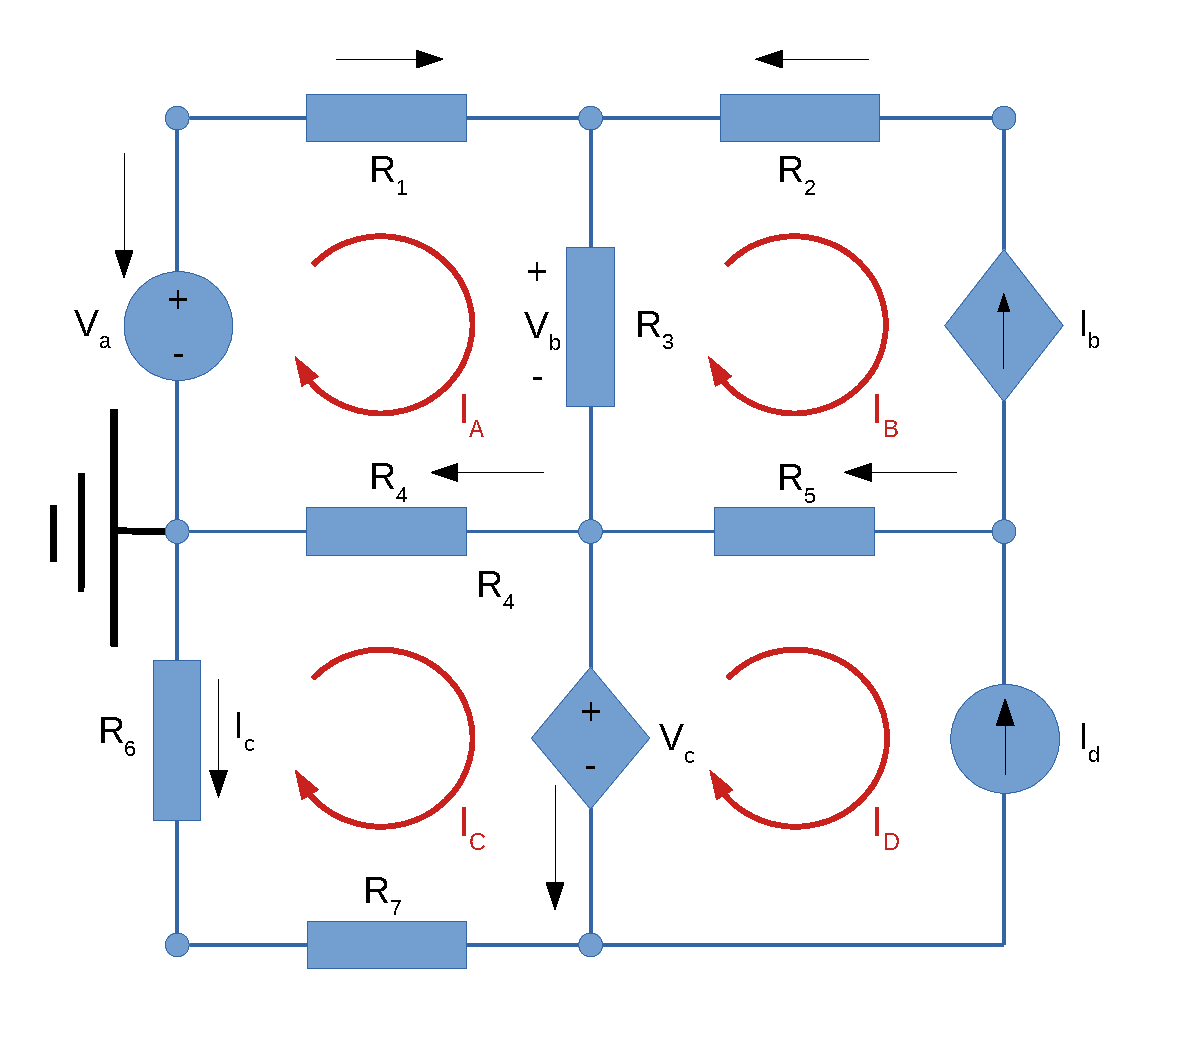
\includegraphics[width=0.5\linewidth]{CircuitMesh.pdf}
\caption{Circuit analysed with mesh currents.}
\label{fig:Circuit_Mesh}
\end{figure}

After identifying the mesh currents, we used the Kirchhoff Voltage Law~(KVL) in the left meshes (Mesh~$\alpha$~ and Mesh~$\delta$~).

\begin{equation}
 V_a= R_1I_a + V_{\beta} + R_4(I_{\alpha} - I_{\delta});
  \label{eq:MM_Alpha}
\end{equation}
\begin{equation}
  R_6I_{\delta} + R_4(I_{\delta} + V_{\delta} + R_7I_{\delta} = 0;
  \label{eq:MM_Delta}
\end{equation}

Besides that we know that I_b=I_{\beta} , I_d=-I_{\gamma} and I_c=-I_{\delta}.

At this point we have 5 equations with 8 unknown variables (I_{\alpha}, I_{\beta}, I_{\delta}, I_b, I_c, I_d, V_{\beta}, V_{\delta}).
It is required more 3 equations that add more information in order to get the same number of unkonwn variables and equations. 
\begin{equation}
 V_{\delta}=K_{\delta}I_{\delta}
  \label{eq:Vc}
\end{equation}
\begin{equation}
  I_{\beta}=K_{\beta}V_{\beta}
  \label{eq:Ib}
\end{equation}
\begin{equation}
V_{\beta}=R_3(I_a-I_b)
\end{equation}


The solution to this linear system of equations is determined by Octave:

\begin{table}[h]
  \centering
  \begin{tabular}{|l|r|}
    \hline    
    {\bf Variables} & {\bf Value [A or V]} \\ \hline
    I_{A} & 1.067284e-03 \\ \hline 
I_{B} & 1.118444e-03 \\ \hline 
I_{C} & 0.000000e+00 \\ \hline 
I_{D} & -1.019408e-03 \\ \hline 
@V_{b} & -1.541489e-01 \\ \hline 
@V_{c} & -0.000000e+00 \\ \hline 
I_{b} & -1.118444e-03 \\ \hline 
I_{c} & -0.000000e+00 \\ \hline 

  \end{tabular}
  \caption{Variables in the Mesh Method. A variable preceded by @ is of type {\em voltage} and expressed in Volts; other variables are of type {\em Current} and expressed in Amps.}
  \label{tab:malhas}
\end{table}

\subsection{Nodal Method}

In this subsection we make use of the other method (Nodal Method) to determinate the values of current and voltage by finding first all the knots in the circuit, as made in Figure \ref{fig:Circuit_Nodal}.

\begin{figure}[H] 
\centering
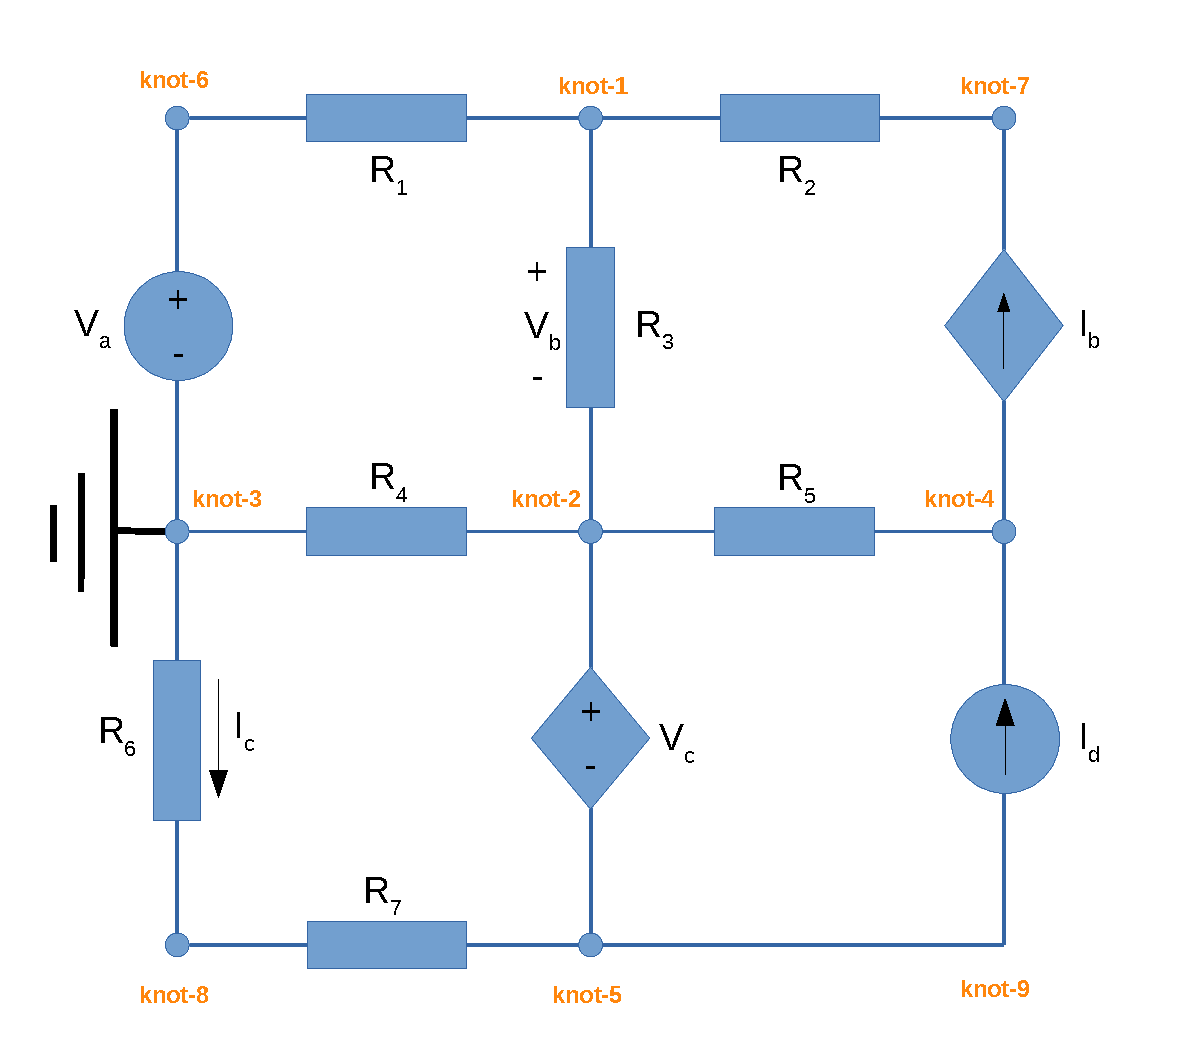
\includegraphics[width=0.5\linewidth]{CircuitNodal.pdf}
\caption{Circuit analysed with nodal voltages.}
\label{fig:Circuit_Nodal}
\end{figure}

After finding all the knots we apply KCL (Kirchhoff Current Law) to all the knots except knots 2, 3, 5 and 6 because they are connected to tension sources.
Note that v_i is a reference to the potencial in knot i.

\begin{equation}
  \frac{v_6-v_1}{R_1} + \frac{v_7-v_1}{R_2} = \frac{V_b}{R_3};
\end{equation}
\begin{equation}
  I_{\beta} = \frac{v_7-v_1}{R_2};	
\end{equation}
\begin{equation}
  I_{\gamma} = \frac{v_4-v_2}{R_5}+I_{\beta};
\end{equation}
\begin{equation}
  I_{\delta} = \frac{v_8-v_5}{R_7};
\end{equation}

We also know that:

\begin{equation}
  V_{\alpha}= v_6-v_3;
\end{equation}
\begin{equation}
  V_{\beta}= v_1-v_2.
\end{equation}
\begin{equation}
  V_{\delta}= v_2-v_5.
\end{equation}

And we have the same equations determinated using Meshes Method:
\begin{equation}
 V_{\beta}=K_{\beta}I_{\beta}
\end{equation}
\begin{equation}
 V_{\delta}=K_{\delta}I_{\delta}
\end{equation}

Using Ohm’s Law, we find the relation:
\begin{equation}
  I_c = \frac{v_3-v_8}{R_6}.
  \label{eq:NM_OhmIc}
\end{equation}

At this point we have 10 equations and 12 unkown variables, so we need 2 more equations that add the information that we need to determinate our final linear system of equations.
We can establish v_2=0 and by continuity of the current in the tension sources we have: 

\begin{equation}
  I_c + \frac{v_6-v_1}{R_1}= \frac{v_2-v_3}{R_4}.
\end{equation}
The solution to this linear system of equations is determined by Octave:

\begin{table}[h]
  \centering
  \begin{tabular}{|l|r|}
    \hline    
    {\bf Name} & {\bf Value [A or V]} \\ \hline
    V_{1} & 3.878423e-05  \\ \hline 
V_{2} & 1.110223e-16  \\ \hline 
V_{3} & -2.255973e-13  \\ \hline 
V_{4} & 1.890796e+01  \\ \hline 
V_{5} & 7.105387e-01  \\ \hline 
V_{6} & 5.230611e+00  \\ \hline 
V_{7} & -1.074709e+01  \\ \hline 
V_{8} & 6.239231e-01  \\ \hline 
V_{b} & 3.878423e-05  \\ \hline 
V_{c} & -7.105387e-01  \\ \hline 
I_{b} & -5.155393e-03  \\ \hline 
I_{c} & -8.618601e-05  \\ \hline 

  \end{tabular}
  \caption{Variables in the Nodal Method. A variable preceded by @ is of type {\em current} and expressed in Ampere; other variables are of type {\em voltage} and expressed in Volt.}
  \label{tab:nos}
\end{table}



\sction{Simulations analysis}
\label{sec:simulation}

\subsection{Operation Point analysis}

Table~\ref{tab:op} shows the simulated operating point results for the circuit
under analysis.

\begin{table}[h]
  \centering
  \begin{tabular}{|l|r|}
    \hline    
    {\bf Name} & {\bf Value [A or V]} \\ \hline
    @gb[i] & -2.92076e-04\\ \hline
@id[current] & 1.019408e-03\\ \hline
@r1[i] & 2.787154e-04\\ \hline
@r2[i] & 2.920757e-04\\ \hline
@r3[i] & -1.33603e-05\\ \hline
@r4[i] & -1.23752e-03\\ \hline
@r5[i] & -1.31148e-03\\ \hline
@r6[i] & 9.588061e-04\\ \hline
@r7[i] & 9.588061e-04\\ \hline
v(1) & 4.947829e+00\\ \hline
v(2) & 4.988084e+00\\ \hline
v(3) & 0.000000e+00\\ \hline
v(4) & 9.004000e+00\\ \hline
v(5) & -2.91655e+00\\ \hline
v(6) & 5.230611e+00\\ \hline
v(7) & 4.338957e+00\\ \hline
v(8) & -1.95296e+00\\ \hline

  \end{tabular}
  \caption{Operating point. A variable preceded by @ is of type {\em current}
    and expressed in Ampere; other variables are of type {\it voltage} and expressed in
    Volt.}
  \label{tab:op}
\end{table}



\section{Conclusion}
\label{sec:conclusion}

In this laboratory assignment the objective of analysing an RC circuit has been
achieved. Static, time and frequency analyses have been performed both
theoretically using the Octave maths tool and by circuit simulation using the
Ngspice tool. The simulation results matched the theoretical results
precisely. The reason for this perfect match is the fact that this is a
straightforward circuit containing only linear components, so the theoretical
and simulation models cannot differ. For more complex components, the
theoretical and simulation models could differ but this is not the case in this
work.

\lipsum[1-1]

%\cleardoublepage

% ----------------------------------------------------------------------
%  Bibliography
% ----------------------------------------------------------------------
%\addcontentsline{toc}{section}{\bibname}
%\bibliographystyle{abbrvunsrtnat} % <<<<< SELECT IF USING REFERENCES BY NUMBER (CITATION ORDER)
%\bibliography{../../../BIBfile.bib}

% ----------------------------------------------------------------------
\end{document}
% ----------------------------------------------------------------------
